\documentclass[tikz]{standalone}

\begin{document}
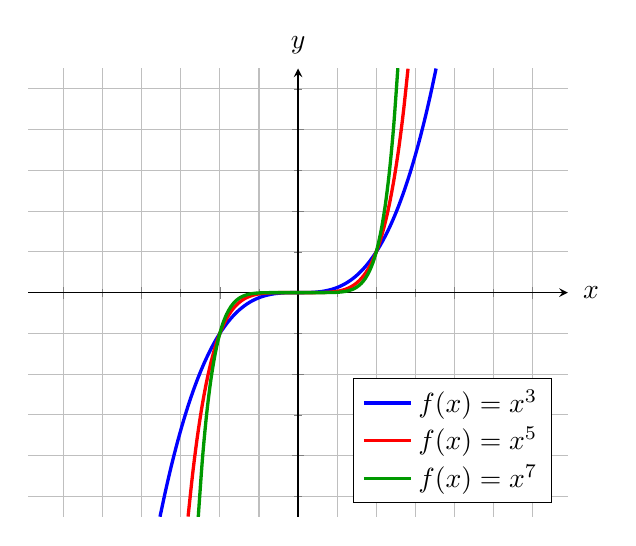
\begin{tikzpicture}
    \begin{axis}[%
        xlabel=$x$, ylabel=$y$, legend pos=south east,
        grid=both, xmin=-3.45, xmax=3.45, ymin=-5.5, ymax=5.5,
        axis lines = middle,
        minor x tick num=1, minor y tick num=1,
        xlabel style = {at={(axis description cs:1.01,0.5)},anchor=west},
        ylabel style = {at={(axis description cs:0.5,1.01)},anchor=south},
        xticklabels = {}, yticklabels={},
    ]
    \addplot[blue, very thick, smooth, samples=50, domain=-1.765:1.765] plot {x^3};
    \addplot[red, very thick, smooth, samples=50, domain=-1.406:1.406] plot {x^5};
    \addplot[green!60!black, very thick, smooth, samples=50, domain=-1.276:1.276] plot {x^7};
    \legend{$f(x)=x^3$,$f(x)=x^5$,$f(x)=x^7$}
    \end{axis}
\end{tikzpicture}
\end{document}
